
%% bare_conf.tex
%% V1.3
%% 2007/01/11
%% by Michael Shell
%% See:
%% http://www.michaelshell.org/
%% for current contact information.
%%
%% This is a skeleton file demonstrating the use of IEEEtran.cls
%% (requires IEEEtran.cls version 1.7 or later) with an IEEE conference paper.
%%
%% Support sites:
%% http://www.michaelshell.org/tex/ieeetran/
%% http://www.ctan.org/tex-archive/macros/latex/contrib/IEEEtran/
%% and
%% http://www.ieee.org/

%%*************************************************************************
%% Legal Notice:
%% This code is offered as-is without any warranty either expressed or
%% implied; without even the implied warranty of MERCHANTABILITY or
%% FITNESS FOR A PARTICULAR PURPOSE! 
%% User assumes all risk.
%% In no event shall IEEE or any contributor to this code be liable for
%% any damages or losses, including, but not limited to, incidental,
%% consequential, or any other damages, resulting from the use or misuse
%% of any information contained here.
%%
%% All comments are the opinions of their respective authors and are not
%% necessarily endorsed by the IEEE.
%%
%% This work is distributed under the LaTeX Project Public License (LPPL)
%% ( http://www.latex-project.org/ ) version 1.3, and may be freely used,
%% distributed and modified. A copy of the LPPL, version 1.3, is included
%% in the base LaTeX documentation of all distributions of LaTeX released
%% 2003/12/01 or later.
%% Retain all contribution notices and credits.
%% ** Modified files should be clearly indicated as such, including  **
%% ** renaming them and changing author support contact information. **
%%
%% File list of work: IEEEtran.cls, IEEEtran_HOWTO.pdf, bare_adv.tex,
%%                    bare_conf.tex, bare_jrnl.tex, bare_jrnl_compsoc.tex
%%*************************************************************************

% *** Authors should verify (and, if needed, correct) their LaTeX system  ***
% *** with the testflow diagnostic prior to trusting their LaTeX platform ***
% *** with production work. IEEE's font choices can trigger bugs that do  ***
% *** not appear when using other class files.                            ***
% The testflow support page is at:
% http://www.michaelshell.org/tex/testflow/



% Note that the a4paper option is mainly intended so that authors in
% countries using A4 can easily print to A4 and see how their papers will
% look in print - the typesetting of the document will not typically be
% affected with changes in paper size (but the bottom and side margins will).
% Use the testflow package mentioned above to verify correct handling of
% both paper sizes by the user's LaTeX system.
%
% Also note that the "draftcls" or "draftclsnofoot", not "draft", option
% should be used if it is desired that the figures are to be displayed in
% draft mode.
%
\documentclass[conference]{IEEEtran}
% Add the compsoc option for Computer Society conferences.
%
% If IEEEtran.cls has not been installed into the LaTeX system files,
% manually specify the path to it like:
% \documentclass[conference]{../sty/IEEEtran}




\usepackage{multirow}
\usepackage{multicol}
\usepackage{graphicx}


% Some very useful LaTeX packages include:
% (uncomment the ones you want to load)


% *** MISC UTILITY PACKAGES ***
%
%\usepackage{ifpdf}
% Heiko Oberdiek's ifpdf.sty is very useful if you need conditional
% compilation based on whether the output is pdf or dvi.
% usage:
% \ifpdf
%   % pdf code
% \else
%   % dvi code
% \fi
% The latest version of ifpdf.sty can be obtained from:
% http://www.ctan.org/tex-archive/macros/latex/contrib/oberdiek/
% Also, note that IEEEtran.cls V1.7 and later provides a builtin
% \ifCLASSINFOpdf conditional that works the same way.
% When switching from latex to pdflatex and vice-versa, the compiler may
% have to be run twice to clear warning/error messages.






% *** CITATION PACKAGES ***
%
\usepackage{cite}
% cite.sty was written by Donald Arseneau
% V1.6 and later of IEEEtran pre-defines the format of the cite.sty package
% \cite{} output to follow that of IEEE. Loading the cite package will
% result in citation numbers being automatically sorted and properly
% "compressed/ranged". e.g., [1], [9], [2], [7], [5], [6] without using
% cite.sty will become [1], [2], [5]--[7], [9] using cite.sty. cite.sty's
% \cite will automatically add leading space, if needed. Use cite.sty's
% noadjust option (cite.sty V3.8 and later) if you want to turn this off.
% cite.sty is already installed on most LaTeX systems. Be sure and use
% version 4.0 (2003-05-27) and later if using hyperref.sty. cite.sty does
% not currently provide for hyperlinked citations.
% The latest version can be obtained at:
% http://www.ctan.org/tex-archive/macros/latex/contrib/cite/
% The documentation is contained in the cite.sty file itself.






% *** GRAPHICS RELATED PACKAGES ***
%
\ifCLASSINFOpdf
  % \usepackage[pdftex]{graphicx}
  % declare the path(s) where your graphic files are
  % \graphicspath{{../pdf/}{../jpeg/}}
  % and their extensions so you won't have to specify these with
  % every instance of \includegraphics
  % \DeclareGraphicsExtensions{.pdf,.jpeg,.png}
\else
  % or other class option (dvipsone, dvipdf, if not using dvips). graphicx
  % will default to the driver specified in the system graphics.cfg if no
  % driver is specified.
  % \usepackage[dvips]{graphicx}
  % declare the path(s) where your graphic files are
  % \graphicspath{{../eps/}}
  % and their extensions so you won't have to specify these with
  % every instance of \includegraphics
  % \DeclareGraphicsExtensions{.eps}
\fi
% graphicx was written by David Carlisle and Sebastian Rahtz. It is
% required if you want graphics, photos, etc. graphicx.sty is already
% installed on most LaTeX systems. The latest version and documentation can
% be obtained at: 
% http://www.ctan.org/tex-archive/macros/latex/required/graphics/
% Another good source of documentation is "Using Imported Graphics in
% LaTeX2e" by Keith Reckdahl which can be found as epslatex.ps or
% epslatex.pdf at: http://www.ctan.org/tex-archive/info/
%
% latex, and pdflatex in dvi mode, support graphics in encapsulated
% postscript (.eps) format. pdflatex in pdf mode supports graphics
% in .pdf, .jpeg, .png and .mps (metapost) formats. Users should ensure
% that all non-photo figures use a vector format (.eps, .pdf, .mps) and
% not a bitmapped formats (.jpeg, .png). IEEE frowns on bitmapped formats
% which can result in "jaggedy"/blurry rendering of lines and letters as
% well as large increases in file sizes.
%
% You can find documentation about the pdfTeX application at:
% http://www.tug.org/applications/pdftex





% *** MATH PACKAGES ***
%
%\usepackage[cmex10]{amsmath}
% A popular package from the American Mathematical Society that provides
% many useful and powerful commands for dealing with mathematics. If using
% it, be sure to load this package with the cmex10 option to ensure that
% only type 1 fonts will utilized at all point sizes. Without this option,
% it is possible that some math symbols, particularly those within
% footnotes, will be rendered in bitmap form which will result in a
% document that can not be IEEE Xplore compliant!
%
% Also, note that the amsmath package sets \interdisplaylinepenalty to 10000
% thus preventing page breaks from occurring within multiline equations. Use:
%\interdisplaylinepenalty=2500
% after loading amsmath to restore such page breaks as IEEEtran.cls normally
% does. amsmath.sty is already installed on most LaTeX systems. The latest
% version and documentation can be obtained at:
% http://www.ctan.org/tex-archive/macros/latex/required/amslatex/math/





% *** SPECIALIZED LIST PACKAGES ***
%
\usepackage{algorithm}
\usepackage{algorithmic}
% algorithmic.sty was written by Peter Williams and Rogerio Brito.
% This package provides an algorithmic environment fo describing algorithms.
% You can use the algorithmic environment in-text or within a figure
% environment to provide for a floating algorithm. Do NOT use the algorithm
% floating environment provided by algorithm.sty (by the same authors) or
% algorithm2e.sty (by Christophe Fiorio) as IEEE does not use dedicated
% algorithm float types and packages that provide these will not provide
% correct IEEE style captions. The latest version and documentation of
% algorithmic.sty can be obtained at:
% http://www.ctan.org/tex-archive/macros/latex/contrib/algorithms/
% There is also a support site at:
% http://algorithms.berlios.de/index.html
% Also of interest may be the (relatively newer and more customizable)
% algorithmicx.sty package by Szasz Janos:
% http://www.ctan.org/tex-archive/macros/latex/contrib/algorithmicx/




% *** ALIGNMENT PACKAGES ***
%
%\usepackage{array}
% Frank Mittelbach's and David Carlisle's array.sty patches and improves
% the standard LaTeX2e array and tabular environments to provide better
% appearance and additional user controls. As the default LaTeX2e table
% generation code is lacking to the point of almost being broken with
% respect to the quality of the end results, all users are strongly
% advised to use an enhanced (at the very least that provided by array.sty)
% set of table tools. array.sty is already installed on most systems. The
% latest version and documentation can be obtained at:
% http://www.ctan.org/tex-archive/macros/latex/required/tools/


%\usepackage{mdwmath}
%\usepackage{mdwtab}
% Also highly recommended is Mark Wooding's extremely powerful MDW tools,
% especially mdwmath.sty and mdwtab.sty which are used to format equations
% and tables, respectively. The MDWtools set is already installed on most
% LaTeX systems. The lastest version and documentation is available at:
% http://www.ctan.org/tex-archive/macros/latex/contrib/mdwtools/


% IEEEtran contains the IEEEeqnarray family of commands that can be used to
% generate multiline equations as well as matrices, tables, etc., of high
% quality.


%\usepackage{eqparbox}
% Also of notable interest is Scott Pakin's eqparbox package for creating
% (automatically sized) equal width boxes - aka "natural width parboxes".
% Available at:
% http://www.ctan.org/tex-archive/macros/latex/contrib/eqparbox/





% *** SUBFIGURE PACKAGES ***
%\usepackage[tight,footnotesize]{subfigure}
% subfigure.sty was written by Steven Douglas Cochran. This package makes it
% easy to put subfigures in your figures. e.g., "Figure 1a and 1b". For IEEE
% work, it is a good idea to load it with the tight package option to reduce
% the amount of white space around the subfigures. subfigure.sty is already
% installed on most LaTeX systems. The latest version and documentation can
% be obtained at:
% http://www.ctan.org/tex-archive/obsolete/macros/latex/contrib/subfigure/
% subfigure.sty has been superceeded by subfig.sty.



%\usepackage[caption=false]{caption}
%\usepackage[font=footnotesize]{subfig}
% subfig.sty, also written by Steven Douglas Cochran, is the modern
% replacement for subfigure.sty. However, subfig.sty requires and
% automatically loads Axel Sommerfeldt's caption.sty which will override
% IEEEtran.cls handling of captions and this will result in nonIEEE style
% figure/table captions. To prevent this problem, be sure and preload
% caption.sty with its "caption=false" package option. This is will preserve
% IEEEtran.cls handing of captions. Version 1.3 (2005/06/28) and later 
% (recommended due to many improvements over 1.2) of subfig.sty supports
% the caption=false option directly:
%\usepackage[caption=false,font=footnotesize]{subfig}
%
% The latest version and documentation can be obtained at:
% http://www.ctan.org/tex-archive/macros/latex/contrib/subfig/
% The latest version and documentation of caption.sty can be obtained at:
% http://www.ctan.org/tex-archive/macros/latex/contrib/caption/




% *** FLOAT PACKAGES ***
%
%\usepackage{fixltx2e}
% fixltx2e, the successor to the earlier fix2col.sty, was written by
% Frank Mittelbach and David Carlisle. This package corrects a few problems
% in the LaTeX2e kernel, the most notable of which is that in current
% LaTeX2e releases, the ordering of single and double column floats is not
% guaranteed to be preserved. Thus, an unpatched LaTeX2e can allow a
% single column figure to be placed prior to an earlier double column
% figure. The latest version and documentation can be found at:
% http://www.ctan.org/tex-archive/macros/latex/base/



%\usepackage{stfloats}
% stfloats.sty was written by Sigitas Tolusis. This package gives LaTeX2e
% the ability to do double column floats at the bottom of the page as well
% as the top. (e.g., "\begin{figure*}[!b]" is not normally possible in
% LaTeX2e). It also provides a command:
%\fnbelowfloat
% to enable the placement of footnotes below bottom floats (the standard
% LaTeX2e kernel puts them above bottom floats). This is an invasive package
% which rewrites many portions of the LaTeX2e float routines. It may not work
% with other packages that modify the LaTeX2e float routines. The latest
% version and documentation can be obtained at:
% http://www.ctan.org/tex-archive/macros/latex/contrib/sttools/
% Documentation is contained in the stfloats.sty comments as well as in the
% presfull.pdf file. Do not use the stfloats baselinefloat ability as IEEE
% does not allow \baselineskip to stretch. Authors submitting work to the
% IEEE should note that IEEE rarely uses double column equations and
% that authors should try to avoid such use. Do not be tempted to use the
% cuted.sty or midfloat.sty packages (also by Sigitas Tolusis) as IEEE does
% not format its papers in such ways.





% *** PDF, URL AND HYPERLINK PACKAGES ***
%
%\usepackage{url}
% url.sty was written by Donald Arseneau. It provides better support for
% handling and breaking URLs. url.sty is already installed on most LaTeX
% systems. The latest version can be obtained at:
% http://www.ctan.org/tex-archive/macros/latex/contrib/misc/
% Read the url.sty source comments for usage information. Basically,
% \url{my_url_here}.





% *** Do not adjust lengths that control margins, column widths, etc. ***
% *** Do not use packages that alter fonts (such as pslatex).         ***
% There should be no need to do such things with IEEEtran.cls V1.6 and later.
% (Unless specifically asked to do so by the journal or conference you plan
% to submit to, of course. )


% correct bad hyphenation here
\hyphenation{op-tical net-works semi-conduc-tor}


\begin{document}
%
% paper title
% can use linebreaks \\ within to get better formatting as desired
\title{CBFB: A Ciphertext Byte Frequency Balancing Mode of Operation for Byte-Oriented Stream Ciphers	}


% author names and affiliations
% use a multiple column layout for up to three different
% affiliations



% conference papers do not typically use \thanks and this command
% is locked out in conference mode. If really needed, such as for
% the acknowledgment of grants, issue a \IEEEoverridecommandlockouts
% after \documentclass

% for over three affiliations, or if they all won't fit within the width
% of the page, use this alternative format:
% 
%\author{\IEEEauthorblockN{Michael Shell\IEEEauthorrefmark{1},
%Homer Simpson\IEEEauthorrefmark{2},
%James Kirk\IEEEauthorrefmark{3}, 
%Montgomery Scott\IEEEauthorrefmark{3} and
%Eldon Tyrell\IEEEauthorrefmark{4}}
%\IEEEauthorblockA{\IEEEauthorrefmark{1}School of Electrical and Computer Engineering\\
%Georgia Institute of Technology,
%Atlanta, Georgia 30332--0250\\ Email: see http://www.michaelshell.org/contact.html}
%\IEEEauthorblockA{\IEEEauthorrefmark{2}Twentieth Century Fox, Springfield, USA\\
%Email: homer@thesimpsons.com}
%\IEEEauthorblockA{\IEEEauthorrefmark{3}Starfleet Academy, San Francisco, California 96678-2391\\
%Telephone: (800) 555--1212, Fax: (888) 555--1212}
%\IEEEauthorblockA{\IEEEauthorrefmark{4}Tyrell Inc., 123 Replicant Street, Los Angeles, California 90210--4321}}




% use for special paper notices
%\IEEEspecialpapernotice{(Invited Paper)}




% make the title area
\maketitle


\begin{abstract}
%\boldmath
This paper introduces a new mode of operation for byte-oriented stream ciphers. This mode of operation, here called CCFB (Ciphertext Byte Frequency Balancing mode), consists of an algorithm that balances out the byte frequency of the ciphertext produced by the stream cipher. The main benefit of its utilization is to make cryptanalysis by means of statistical byte frequency examination of the ciphertext more difficult for potential attackers producing, therefore, more secure communications at the expense of some performance overhead added to the ciphering/deciphering procedures.
\end{abstract}
% IEEEtran.cls defaults to using nonbold math in the Abstract.
% This preserves the distinction between vectors and scalars. However,
% if the conference you are submitting to favors bold math in the abstract,
% then you can use LaTeX's standard command \boldmath at the very start
% of the abstract to achieve this. Many IEEE journals/conferences frown on
% math in the abstract anyway.

% no keywords




% For peer review papers, you can put extra information on the cover
% page as needed:
% \ifCLASSOPTIONpeerreview
% \begin{center} \bfseries EDICS Category: 3-BBND \end{center}
% \fi
%
% For peerreview papers, this IEEEtran command inserts a page break and
% creates the second title. It will be ignored for other modes.
\IEEEpeerreviewmaketitle



\section{Introduction}
% no \IEEEPARstart

The main purpose of the use of cryptography is to keep information confidential, that is, to protect information from non-authorized access by transforming the plaintext into ciphertext and then allowing authorized users to recover the plaintext from the ciphertext. All of this is accomplished by means of cryptosystems composed of ciphering/deciphering algorithms and one or more keys. There is continuous advancement in the world of cryptography and new algorithms are constantly emerging. Evolution in this field of knowledge is followed closely by the progress of cryptanalysis, which refers to the study of cryptosystems with a view of finding weaknesses in them that might facilitate the retrieval of the plaintext from the ciphertext, without necessarily knowing the key(s) or the algorithm.

One of the most well-known methods used in cryptanalysis is the statistical analysis of the byte frequency of a ciphered message. Although this approach was primarily used with classical ciphers, such as the Caesar and Vigenère ciphers \cite{william-stallings}, to exploit the character frequency that is inherent to a given written language, it has been extended and applied to cryptanalyze modern block ciphers such as DES \cite{nist,feng} and AES \cite{aes, vaudenay}, as well as to modern stream ciphers such as RC4 \cite{rivest, gaithuru, fluhrer}, SNOW \cite{ekdahl, ekdahl2} and Loiss \cite{feng, gupta}. In fact, statistical analysis can be applied generically in the cryptanalysis of both block ciphers \cite{filiol, junod} [13, 14] and stream ciphers \cite{englund, fischer,bokhari}.  

This research presents a mode of operation, particularly applicable to byte-oriented stream ciphers, which is able to balance out the byte frequency of the produced ciphertext. This mode of operation is shown to be suitable to be implemented with any byte-oriented stream cipher simply by “enveloping” it with an additional algorithmic layer that enforces a balanced byte frequency distribution in terms of the possible values of the generated ciphertext output. 

Therefore, the main contribution of this work is to offer a counter measure to cryptanalytic attacks which attempt to gain insight into a given stream ciphering technique by using byte frequency analysis. 
The remainder of this paper is organized as follows. Section 2 contains some background material intended to make the paper as self-contained as possible. Section 3 describes the byte frequency balancing algorithm and is the core of the paper. Section 4 discusses a particular implementation of the byte frequency balancing algorithm applied to the RC4 stream cipher and analyzes the implementation results. Finally, Section 5 presents concluding remarks.


%This demo file is intended to serve as a ``starter file''
%for IEEE conference papers produced under \LaTeX\ using
%IEEEtran.cls version 1.7 and later.
% You must have at least 2 lines in the paragraph with the drop letter
% (should never be an issue)
%I wish you the best of success.

%\hfill mds
 
%\hfill January 11, 2007

\section{Background}

There are two main types of cryptosystems: symmetric key cryptosystems and asymmetric key cryptosystems. A symmetric key cryptosystem uses the same key to encrypt the plaintext and to decrypt the corresponding ciphertext. An asymmetric key cryptosystem uses a pair of keys, correlated to one another in some mathematical way, such that one of the keys is used to encrypt the plaintext, while the other is used to decrypt the produced ciphertext. The work presented in this paper focuses on symmetric key cryptosystems. 

Symmetric key cryptosystems may use block ciphering/deciphering algorithms or stream ciphering/deciphering algorithms. 

Block ciphers encrypt/decrypt an entire block of characters/bytes in a single operation, where the size of each block is predefined. The plaintext is processed block by block in the encryption procedure, as well as in the decryption procedure. Well-known block ciphers are the Data Encryption Standard (DES), developed by IBM, and the Advanced Encryption Standard (AES), developed by two Belgian cryptographers, Joan Daemen and Vincent Rijmen.

Stream ciphers can be bit-oriented, byte-oriented or word-oriented, depending on whether they encrypt/decrypt the plaintext/ciphertext one bit, one byte or one word at a time. The work presented in this paper finds its applicability in the scope of byte-oriented stream ciphers, although it could be extended to word-oriented stream ciphers as well.

\subsection{Byte-oriented stream ciphers}

The overall behavior of a byte-oriented stream cipher includes the generation of a pseudorandom byte keystream (a byte stream generated from a key) and an encryption/decryption function. At the sender side the encryption function, usually an exclusive-or operation, takes as inputs the sequence of bytes of a plaintext, plus the generated pseudorandom byte stream, and produces the corresponding ciphered byte sequence. At the receiver side the same keystream must be again generated and the exclusive-or operation once more applied to the ciphertext sequence to recover the plaintext. The keystream utilized by the stream cipher must come from a pseudorandom number generator, since it must be exactly reproduced in the receiver side in order for the plaintext to be recovered from the ciphertext.

Nowadays, there are four stream ciphering algorithms that cover 80\% of the world telecommunication and cyber space. They are: A5/1, A5/2, E0 and RC4 [18].

This paper presents an application of the proposed byte frequency balancing algorithm to the RC4 byte-oriented stream cipher. RC4 was chosen because of its widespread acceptance and because it is considered the fastest stream cipher available. The following section briefly explains how RC4 works.


\subsubsection{The RC4 byte-oriented stream cipher}

RC4 \cite{william-stallings, gaithuru} was designed by Ron Rivest in 1987 and is widely used, because of its simplicity and high performance, with network protocols such as SSL, TLS, WEP, and WPA, as well as with applications like Microsoft Windows, Lotus Notes, Apple AOCE, Oracle and Secure SQL, among others. 

RC4 is based on the permutation of the values of a 256-byte state vector S. At first S undergoes an initialization procedure based on a variable sized key K. After initialization a byte generation procedure is executed on S which, at each step, scrambles the bytes of S and produces an output byte bo. This output byte is then used to cipher the next plaintext byte using an exclusive-OR operation. The byte generation procedure is essentially a pseudorandom number generator. Figure \ref{rc4-functioning} shows the functional operation of RC4 (ciphering and deciphering) including the following procedures: key initialization, the pseudorandom byte stream generation and the encryption operation.

\begin{figure}[!t]
	\centering
	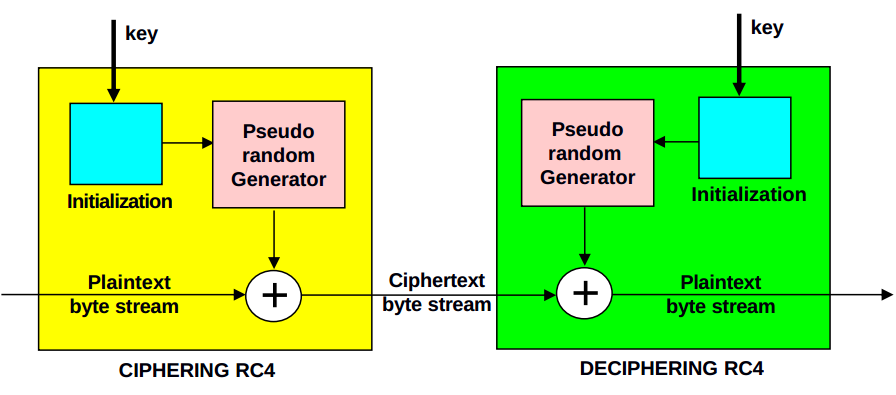
\includegraphics[scale=0.3]{figure1}
	\caption{RC4 functional block description}
	\label{rc4-functioning}
\end{figure}

The key initialization and the pseudorandom byte stream generation procedures are further explained in the next sections.

\paragraph{Key initialization}

RC4 accepts a key with a length keylen between 1 and 256. At initialization time, the state vector S is given initial values S[0] = 0, S[1] = 1, S[2] = 2, ..., S[255] = 255, and a temporary 256-byte vector T is created and initialized with the values of the key K. If K has size 256 bytes, T is made equal to K. If the key is less than 256 bytes, the key is repeated until all 256 positions of T are initialized. This can be more formally expressed as:

\begin{algorithm}
\caption{Initialization}
\begin{algorithmic} 
\FOR{$i=0$ to $255$}
\STATE $S[i] = i$
\STATE $T[i] = K[i \bmod\; keylen]$
\ENDFOR
\end{algorithmic}
\end{algorithm}

The temporary vector T is then used to drive a comprehensive permutation on the bytes of the state vector S. This permutation uses two control variables i and j, taking from 0 to 255, and is performed according to the following pseudo code:

\begin{algorithm}
\caption{Permutation}
\begin{algorithmic} 
\STATE $j = 0$
\FOR{$i=0$ to $255$}
\STATE $j = (j\; + S[i]\; + T[i]) \bmod 256$
\STATE $swap (S[i]\;, S[j])$
\ENDFOR
\end{algorithmic}
\end{algorithm}

\paragraph{The pseudorandom byte stream generation procedure}

After initialization, a stepwise byte stream generation procedure is performed using the state vector S and control variables i, j and k. The control variables i and j and both initialized to 0. Each step of the byte generation procedure permutes a couple of values of S and produces an output byte bo according to the following:

\begin{algorithm}
\caption{Generation}
\begin{algorithmic} 
\STATE $i = (i + 1) \bmod 256$ \COMMENT{generate a new value of i}
\STATE $j = (j + S[i]) \bmod 256$ \COMMENT{generate a new value of j}
\STATE $swap (S[i], S[j])$ \COMMENT{swap two values of S, S[i] and S[j]}
\STATE $k = (S[i] + S[j]) \bmod 256$ \COMMENT{generate the output byte index k}
\STATE $bo = S[k]$ \COMMENT{generate the output byte}
\end{algorithmic}
\end{algorithm}

The byte generation procedure is performed while there are bytes of the plaintext to be ciphered.

\section{CBFB: The Ciphertext Byte Frequency Balancing Algorithm}

This section presents the byte frequency balancing algorithm, details of its operation and advantages of its use.

The CBFB algorithm offers a counter measure to cryptanalytic attacks which attempt to gain insight into a given byte-oriented stream ciphering technique by means of byte frequency analysis. This algorithm may be used with any byte-oriented stream cipher by “enveloping” it with a byte frequency balancing procedure, which causes the ciphered byte stream to be balanced in terms of all its  possible output values.

The mechanism that produces the balanced ciphertext causes the ciphered output to be in the form of rounds of 256 bytes. In each output round each of the 256 possible byte values appears exactly once.  Since each output round is perfectly balanced, the overall ciphertext will also be perfectly balanced in regards to the 256 possible byte values. Obviously, the order in which the 256 byte values appear will be different for each output round. There will be 256! different 256-byte sequences that constitute building blocks for the ciphertext output which can be intermingled in a unimaginably large number of possible repetition and sequence patterns.

A 256-byte table, called the CBFB table, is used to ensure that the byte frequency of the ciphertext is balanced in the manner that follows. In the beginning of a round, all 256 positions in the table are marked as NOT-TAKEN. For each byte of the plaintext to be ciphered the enveloping procedure calls the basic stream ciphering algorithm, having the plaintext byte value as input. The basic stream ciphering algorithm returns what we call a pre-ciphered byte value. After receiving the pre-ciphered byte value, the enveloping algorithm checks the 256-byte round table whether the corresponding entry is already taken (in this round). If that position is not yet taken the pre-ciphered value is accepted as the correct ciphered value for the plaintext at hand, that is, the ciphering procedure for this particular plaintext byte is considered to be successful. Then that round table position is marked as TAKEN, and the ciphered value is sent to the communication channel to the receiving party as part of the ciphertext stream. 

In case the pre-ciphered value position is already taken in the table, the enveloping procedure calls the basic stream ciphering algorithm once more, with the same plaintext byte as input, and again examines the returned value against the round table. This procedure is repeated until a pre-ciphered value is obtained (for that particular plaintext byte) whose position in the round table is not yet taken. When this happens, the corresponding position in the table is marked as TAKEN, and what is sent to the receiving party is:

\begin{enumerate}
	\item A control (or signaling) value to inform the receiving side that conflicts did happen (the value 0 can be used for this purpose); 
	\item The number of attempts minus 1, called delta, (sent as a ciphered byte value) incurred by the ciphering procedure before generating a ciphered byte value that corresponded to a NOT-TAKEN position in the round table. It should be noticed that an additional invocation to the basic stream ciphering algorithm will be needed in order to cipher the delta value.
	\item The finally accepted ciphered byte value. 
\end{enumerate}

This process continues until the round is completed (that is, when all positions in the table are taken). When that happens, the round table is reset and another round starts over. The entire process continues while there are still plaintext bytes to be ciphered.

On the receiving side, the deciphering enveloping algorithm has no need to use a balancing round table. When a ciphertext byte is received, the enveloping deciphering procedure invokes the basic stream ciphering algorithm and obtains the corresponding plaintext byte. If the received byte value is the signaling byte (and, therefore, not a ciphertext byte), the deciphering procedure knows that: 

\begin{enumerate}
	\item he next byte in the incoming byte stream carries the number of conflicts delta until a byte value corresponding to a vacant position in the round table was produced by the ciphering procedure on the sending side. The deciphering procedure invokes the basic stream ciphering algorithm presenting as input the ciphered delta value to obtain the value of delta.
	\item The byte coming after the (ciphered) delta byte in the incoming byte stream is the ciphertext byte which needs to be deciphered.
\end{enumerate}

For the deciphering enveloping procedure, delta + 1 is the number of invocations to the basic stream ciphering algorithm (after deciphering the delta value)  that are necessary to obtain the correct plaintext byte corresponding to the particular ciphertext byte being deciphered. 

Figure \ref{rc4-cbfb-algorithm} graphically compares the operation of the plain RC4 stream cipher and RC4 “enveloped” by the CBFB algorithm from an input/output perspective. In both cases, from an outside observer viewpoint, the inputs and outputs are the same. The inputs are: a key and an incoming byte stream IBk (Input Bytes, 1 ≤ k ≤ n), while the output is an outcoming byte srtream OBk (Output Bytes, 1 ≤ k ≤ n). A view of the CBFB internals is also shown, in which the CBFB “envelope” invokes the RC4 algorithm delta+1 times (where delta ≥ 0) in order to cipher (decipher) a given input plaintext (ciphertext) byte. In each of these delta+1 invocations the input byte offered to RC4 is always IBk, until the output byte Obj (0 ≤  j ≤  delta) produced by RC4 is the intended OBk. In the ciphering procedure, the intended OBk is the first byte value that is still not taken in the CBFB table. In the deciphering procedure the value of delta is known (from the ciphering side) and the intended OBk is the plaintext byte value corresponding to the ciphertext byte value IBk.

\begin{figure}[!t]
	\centering
	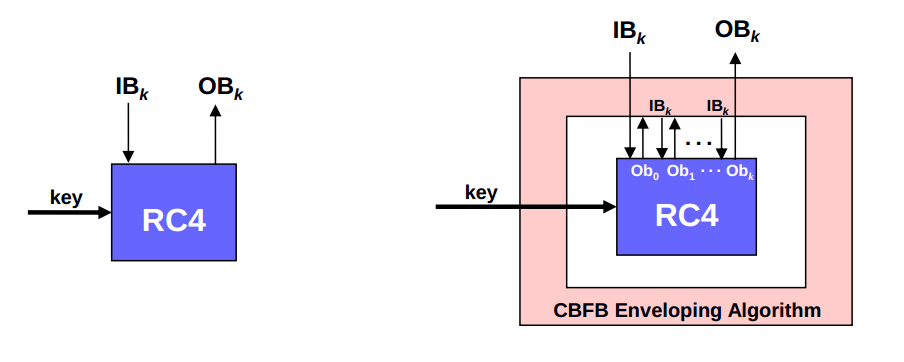
\includegraphics[scale=0.3]{figure2.png}
	\caption{The plain RC4 algorithm and the CBFB "enveloped" RC4}
	\label{rc4-cbfb-algorithm}
\end{figure}


\section{Implementation and Discussion of Experimental Results}

We implemented the CBFB “enveloped” RC4 algorithm according to the description in the previous section, as shown in Figure 2, and compared its performance with the basic RC4 stream cipher for various sizes of the plaintext. 

The next subsections present the implementation architecture, describe our experiments and discuss the obtained results.

\subsection{Implementation architecture}

Figure \ref{architecture} shows the implementation architecture of our experiments. A ciphering and a deciphering instances of the CBFB “enveloped” RC4 stream cipher were deployed in two geographically distinct nodes running Linux Ubuntu connected through a communication network. The network protocol used for the communication of these two nodes was TCP/IP implemented with synchronous Linux sockets.

\begin{figure}[!t]
	\centering
	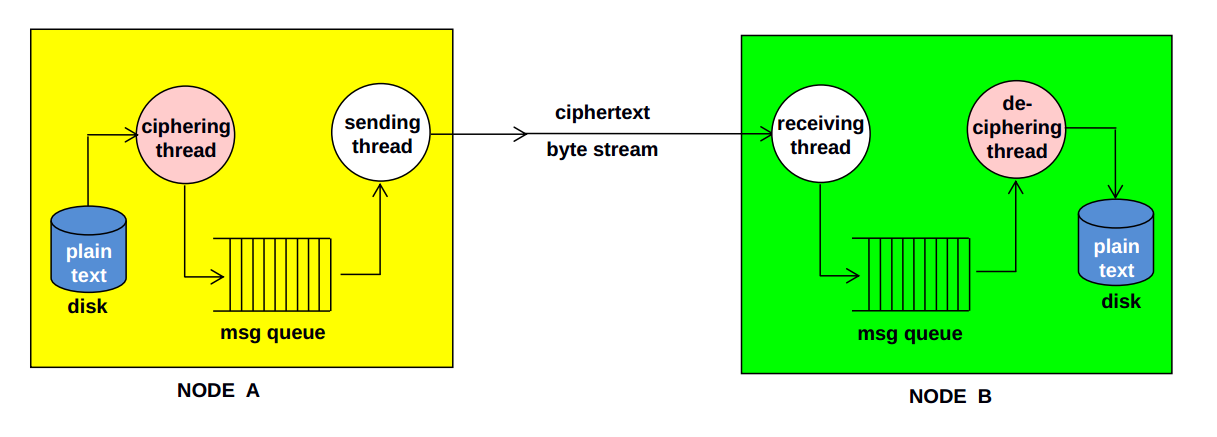
\includegraphics[scale=0.20]{figure3.png}
	\caption{The implementation architecture}
	\label{architecture}
\end{figure}

Two POSIX threads and a message queue were utilized in this implementation. In the sending node (node A in Figure 3) , the ciphering thread reads the plaintext file from the disk, ciphers it using the CBFB “enveloped” RC4 and places the ciphered bytes in the message queue. The sending thread reads the ciphertext from the message queue and sends it through the communication channel. In the receiving node (node B in Figure 3), the receiving thread reads the ciphertext from the communication channel and places it into the message queue. Finally, the deciphering thread reads it from the message queue, deciphers it using the same pseudorandom byte stream provided by the basic RC4 (obtained using the same key) it and writes the resulting plaintext back into disk.

\subsection{Discussion of experimental results}

The ciphering/deciphering experiments were conducted using plaintext files varying from 10 thousands to 1 million characters. 

\begin{table}[!t]
\centering
\begin{tabular}{|c|c|c|}
\hline
Text size(chars) & \# of conflicts & Avg. conflict resolution(ms) \\ \hline
10,000  & 5,036 & 0.001986                                                               \\ \hline
50,000  & 25,167 & 0.001351                                                                 \\ \hline
100,000 & 50,019 & 0.001337                                                                \\ \hline
500,000 & 250,077 & 0.001184                                                                 \\ \hline
1,000,000 & 449,890 & 0.001228                                                               \\ \hline
\end{tabular}
\caption{Ciphering number of conflicts and conflict resolution time}
\label{conflict-amount}
\end{table}

\begin{table}[!t]
\centering
\begin{tabular}{|c|c|c|c|}
\hline
Text size(chars) & RC4(ms) & RC4 + CBFB(ms) & Time overhead(ms) \\ \hline
10,000                                                      & 8        & 14  & 6                                                         \\ \hline
50,000                                                      & 24       & 45  & 21                                                          \\ \hline
100,000                                                     & 36       & 86  &  50                                                         \\ \hline
500,000                                                     & 168      & 409  &  241                                                        \\ \hline
1,000,000                                                   & 292      & 829  &  537                                                        \\ \hline
\end{tabular}
\caption{Ciphering time comparison}
\label{ciphering-time-comparison}
\end{table}

Table \ref{conflict-amount} and \ref{ciphering-time-comparison} compares the ciphering times taken by the CBFB “enveloped” RC4 algorithm with the ciphering times required by the plain RC4 algorithm for the chosen plaintext files. It also shows the number of conflicts the CBFB algorithm had to handle, as well as the average conflict resolution times, when balancing out the ciphertext byte frequency in the ciphering procedure of the various files. It can be observed that the number of conflicts was roughly equal to half the size of the plaintext being encoded. Conversely, the average conflict resolution time for plaintext files of size 10,000 characters or more did not vary significantly.

\begin{table}[!t]
\centering
\begin{tabular}{|c|c|c|c|c|}
\hline
\multirow{2}{*}{\begin{tabular}[c]{@{}c@{}}Text size\\ (chars)\end{tabular}} & \multirow{2}{*}{RC4 (ms)} & \multirow{2}{*}{RC4 + CBFB (ms)} & \multicolumn{2}{c|}{\begin{tabular}[c]{@{}c@{}}Time\\ overhead\end{tabular}} \\ \cline{4-5} 
                                                                             &                           &                                  & ms                                    & \%                                   \\ \hline
10,000                                                                       & 125.2                     & 127.6                            & 2.4                                   & 1.91                                 \\ \hline
50,000                                                                       & 605.9                     & 623.0                            & 17.1                                  & 2.82                                 \\ \hline
100,000                                                                      & 1,144.8                   & 1,214.6                          & 69.8                                  & 6.09                                 \\ \hline
500,000                                                                      & 5,730.0                   & 6,042.2                          & 312.2                                 & 5.44                                 \\ \hline
1,000,000                                                                    & 11,429.6                  & 12,048.7                         & 619.1                                 & 5.42                                 \\ \hline
\end{tabular}
\caption{End-to-end Time Comparison}
\label{end-to-end}
\end{table}

Table \ref{end-to-end} displays the end-to-end times for ciphering and deciphering the various plaintext files using the CBFB “enveloped” RC4 and the plain RC4 algorithm. It can be noticed that the time overhead for the end-to-end encoding/decoding procedure when the CBFB mode of operation is employed between remote communication entities, as compared to the plain RC4 stream cipher, is at most 6.09\% for the architecture and assumptions used in the experiment. The reason for the small variation in the end-to-end times observed in this experiment is that the communication times outweigh the ciphering/deciphering times and, therefore, the processing overhead incurred by CBFB mode of operation is lessened by the communication overhead and the concurrency between processing and communication functionalities afforded by the multithreaded implementation.

% An example of a floating figure using the graphicx package.
% Note that \label must occur AFTER (or within) \caption.
% For figures, \caption should occur after the \includegraphics.
% Note that IEEEtran v1.7 and later has special internal code that
% is designed to preserve the operation of \label within \caption
% even when the captionsoff option is in effect. However, because
% of issues like this, it may be the safest practice to put all your
% \label just after \caption rather than within \caption{}.
%
% Reminder: the "draftcls" or "draftclsnofoot", not "draft", class
% option should be used if it is desired that the figures are to be
% displayed while in draft mode.
%
%begin{figure}[!t]
%\centering
%\includegraphics[width=2.5in]{myfigure}
% where an .eps filename suffix will be assumed under latex, 
% and a .pdf suffix will be assumed for pdflatex; or what has been declared
% via \DeclareGraphicsExtensions.
%\caption{Simulation Results}
%\label{fig_sim}
%\end{figure}

% Note that IEEE typically puts floats only at the top, even when this
% results in a large percentage of a column being occupied by floats.


% An example of a double column floating figure using two subfigures.
% (The subfig.sty package must be loaded for this to work.)
% The subfigure \label commands are set within each subfloat command, the
% \label for the overall figure must come after \caption.
% \hfil must be used as a separator to get equal spacing.
% The subfigure.sty package works much the same way, except \subfigure is
% used instead of \subfloat.
%
%\begin{figure*}[!t]
%\centerline{\subfloat[Case I]\includegraphics[width=2.5in]{subfigcase1}%
%\label{fig_first_case}}
%\hfil
%\subfloat[Case II]{\includegraphics[width=2.5in]{subfigcase2}%
%\label{fig_second_case}}}
%\caption{Simulation results}
%\label{fig_sim}
%\end{figure*}
%
% Note that often IEEE papers with subfigures do not employ subfigure
% captions (using the optional argument to \subfloat), but instead will
% reference/describe all of them (a), (b), etc., within the main caption.


% An example of a floating table. Note that, for IEEE style tables, the 
% \caption command should come BEFORE the table. Table text will default to
% \footnotesize as IEEE normally uses this smaller font for tables.
% The \label must come after \caption as always.
%
%\begin{table}[!t]
%% increase table row spacing, adjust to taste
%\renewcommand{\arraystretch}{1.3}
% if using array.sty, it might be a good idea to tweak the value of
% \extrarowheight as needed to properly center the text within the cells
%\caption{An Example of a Table}
%\label{table_example}
%\centering
%% Some packages, such as MDW tools, offer better commands for making tables
%% than the plain LaTeX2e tabular which is used here.
%\begin{tabular}{|c||c|}
%\hline
%One & Two\\
%\hline
%Three & Four\\
%\hline
%\end{tabular}
%\end{table}


% Note that IEEE does not put floats in the very first column - or typically
% anywhere on the first page for that matter. Also, in-text middle ("here")
% positioning is not used. Most IEEE journals/conferences use top floats
% exclusively. Note that, LaTeX2e, unlike IEEE journals/conferences, places
% footnotes above bottom floats. This can be corrected via the \fnbelowfloat
% command of the stfloats package.



\section{Conclusion}

We have proposed a mode of operation for byte-oriented stream ciphers called CBFB, Ciphertext Byte Frequency Balancing mode.

CBFB undertakes to balance out the ciphertext produced by a stream cipher by evenly distributing the frequency of appearance of all possible output values. The advantage of its use lies in hardening, for a potential attacker, the task of gaining insight into the operation of a particular stream cipher by means of statistical analysis.

Experiments were conducted using the proposed mode of operation with the RC4 stream cipher and showed that the ciphering procedure using CBFB sustains considerable time increase. However, when used between remotely located sender and receiver, the communication times are likely to mask the processing overhead, justifying its use, given the additional security provided. All in all, the idea seems promising and has the potential of being employed with different existing byte-oriented stream ciphers to secure synchronous communications between remote entities. 

Among the possibilities of future work we consider the optimization of the proposed algorithm, possibly by intertwining it with the stream cipher implementation, the extension of the idea to word-oriented stream ciphers and the investigation of the applicability of similar principles to block ciphers such as DES and AES.


% trigger a \newpage just before the given reference
% number - used to balance the columns on the last page
% adjust value as needed - may need to be readjusted if
% the document is modified later
%\IEEEtriggeratref{8}
% The "triggered" command can be changed if desired:
%\IEEEtriggercmd{\enlargethispage{-5in}}

% references section

% can use a bibliography generated by BibTeX as a .bbl file
% BibTeX documentation can be easily obtained at:
% http://www.ctan.org/tex-archive/biblio/bibtex/contrib/doc/
% The IEEEtran BibTeX style support page is at:
% http://www.michaelshell.org/tex/ieeetran/bibtex/
%\bibliographystyle{IEEEtran}
% argument is your BibTeX string definitions and bibliography database(s)
%\bibliography{IEEEabrv,../bib/paper}
%
% <OR> manually copy in the resultant .bbl file
% set second argument of \begin to the number of references
% (used to reserve space for the reference number labels box)
\begin{thebibliography}{1}

\bibitem{william-stallings}
	William Stallings, \emph{Cryptography and network security – Principles and practice}, 6th~ed.\hskip 1em plus
  0.5em minus 0.4em\relax Pearson, 2014.
  
\bibitem{nist}
National Bureau of Standards (today, National Institute of Standards and Technology), \emph{Data Encryption Standard}, FIPS Publication 46.\hskip 1em plus
  0.5em minus 0.4em\relax 1977.
  
\bibitem{aes}
Daemen and V. Rijmen, \emph{The Design of Rijndael: AES – The Advanced Encryption Standard}.\hskip 1em plus
  0.5em minus 0.4em\relax Springer, 2002.
  
\bibitem{rivest}
	R.L. Rivest, \emph{The RC4 Encryption Algorithm}.\hskip 1em plus
  0.5em minus 0.4em\relax RSA Data Security, Inc., 1992.
  
\bibitem{ekdahl}
Patrick Ekdahl, and Thomas Johansson \emph{SNOW – A new stream cipher}.\hskip 1em plus
  0.5em minus 0.4em\relax Proc. of the 1st Open NESSIE Workshop, Heverlee, Belgium, 2000, pp. 167-168.

\bibitem{ekdahl2}
Patrick Ekdahl, and Thomas Johansson \emph{A new version of the stream cipher SNOW}.\hskip 1em plus
  0.5em minus 0.4em\relax Selected Areas in Cryptography, Springer Berlin Heidelberg, 2003, pp. 47-61.
  
\bibitem{feng}
Dengguo Feng, et al. \emph{Loiss: A byte-oriented stream cipher}.\hskip 1em plus
  0.5em minus 0.4em\relax Coding and Cryptology, Springer Berlin Heidelberg, 2011, pp. 109-125.
  
\bibitem{vaudenay}
Serge Vaudenay \emph{An experiment on DES statistical cryptanalysis}.\hskip 1em plus
  0.5em minus 0.4em\relax Proceedings of the 3rd ACM conference on Computer and communications security. ACM, 1996.

\bibitem{gaithuru}
  Juliet N. Gaithuru, and Majid M. Bakhtiari \emph{Statistical analysis of S-Box in Rijndael-AES algorithm and formulation of an enhanced S-Box}.\hskip 1em plus
  0.5em minus 0.4em\relax Journal of Information Assurance \& Security 9.4, 2014.
  
\bibitem{fluhrer}
  Scott R. Fluhrer, and David A. McGrew \emph{Statistical analysis of the alleged RC4 keystream  generator,}.\hskip 1em plus
  0.5em minus 0.4em\relax Fast Software Encryption, Springer Berlin Heidelberg, 2001, pp. 19-30.
  
\bibitem{gupta}
  Sourav Sen Gupta, et al. \emph{(Non-) random sequences from (non-) random permutations Analysis of RC4 stream cipher}.\hskip 1em plus
  0.5em minus 0.4em\relax Journal of Cryptology 27.1, 2014, pp. 67-108.
  
\bibitem{biryukov}
  Alex Biryukov, Aleksandar Kircanski, and Amr M. Youssef. \emph{Cryptanalysis of the Loiss stream cipher}.\hskip 1em plus
  0.5em minus 0.4em\relax Selected Areas in Cryptography, Springer Berlin Heidelberg, 2013.
  
\bibitem{filiol}
  Eric Filiol. \emph{A new statistical testing for symmetric ciphers and hash functions}.\hskip 1em plus
  0.5em minus 0.4em\relax Information and Communications Security, Springer Berlin Heidelberg, 2002, pp. 342-353.
  
\bibitem{junod}
  Pascal Junod. \emph{Statistical cryptanalysis of block ciphers}.\hskip 1em plus
  0.5em minus 0.4em\relax Doctoral dissertation, École Polytechnique Féderale de Lausanne, 2005.
  
\bibitem{englund}
  Häkan Englund, Thomas Johansson, and Meltem Sönmez Turan. \emph{A framework for chosen IV statistical analysis of stream ciphers}.\hskip 1em plus
  0.5em minus 0.4em\relax Progress in Cryptology–INDOCRYPT 2007, Springer Berlin Heidelberg, 2007, pp. 268-281.
  
\bibitem{fischer}
  Simon Fischer, Shahram Khazaei, and Willi Meier, \emph{Chosen IV statistical analysis for key recovery attacks on stream ciphers}.\hskip 1em plus
  0.5em minus 0.4em\relax Progress in Cryptology–AFRICACRYPT 2008. Springer Berlin Heidelberg, 2008. 236-245.
  
\bibitem{bokhari}
  U. Bokhari, Shadab Alam, and Faheem Syeed Masoodi, \emph{Cryptanalysis techniques for stream ciphers: a survey}.\hskip 1em plus
  0.5em minus 0.4em\relax International Journal of Computer Applications 60.9, 2012.
  
\bibitem{bakhtiari}
  Majid Bakhtiari, and Mohd Aizaini Maarof, , \emph{An Efficient Stream Cipher Algorithm for Data Encryption}.\hskip 1em plus
  0.5em minus 0.4em\relax International Journal of Computer Science Issues, Vol. 8, Issue 3, No. 1, May 2011.

\end{thebibliography}




% that's all folks
\end{document}


